\chapter{Jet Algorithms for the L1 Trigger Upgrade}
\label{chap:l1jets}


\subsection{\sc Algorithms for L1 jet reconstruction}
\label{Sec:Algo}
In this section we describe in detail the proposed algorithm to reconstruct, filter, 
and calibrate L1 jets.
We assume that all L1 calorimetric information for a single event is available at 
the same time in the same place. This would be possible with the time multiplexted trigger approach (TMT) \cite{TMT}.


\begin{itemize}

\item {\bf Jet Reconstruction} \\
The proposed jet algorithm builds jets from the outputs of the L1 calorimeter towers, thereby
exploiting the full granularity of the CMS calorimeter. 
In the electromagnic calorimeter (ECAL) one tower consists of $5 \times 5$ 
lead tungstate crystals and in the hadronic calorimeter one block of brass scintillor. 
In the centre of the detector, a tower covers a region of $0.087\times0.087$ in the $\eta-\phi$ plane with the $\eta$ dimension increasing as $\eta$ increases, see \cite{CMSdetector}.
The ECAL and HCAL energy in each tower is summed and these 'L1CaloTowers' are the input to the algorithm. 

A jet consisting of $n \times n$ towers is built at each tower site (See Figure \ref{slide}); 
the algorithm is a sliding window across the calorimeter.
Those jets with a non null energy are saved. 
The resulting numerous overlapping jets are sorted and filtered.

\begin{figure}[h]
%\vspace{-1.cm}
\begin{center}
  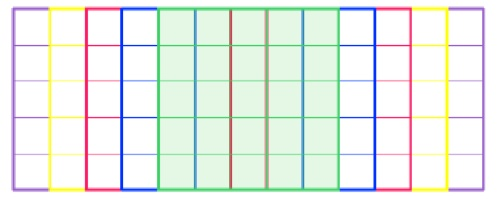
\includegraphics[scale=0.37]{Figures/l1jets/JetOverlaps.jpg}

\caption{Overlaps of 5$\times$5 jet in 1D. A jet is built at each tower on the calorimeter}
\label{slide}
\end{center}
\end{figure}

\item  {\bf Tunable Parameters} \\
Jets are built from a flexible map of calorimeter towers;
the jet shape and size can be set. 
Currently they can be circular or square, although there is scope for any desired shape.
The size can be set to $n$ towers. 
For circular jets this size represents the length of the diameter, 
for square jets it represents the length of the side. 
In previous studies diameter 8 circular jets gave the best angular resolution, so these are presented here. 

With the TMT it is technically possible to build two different L1 jet collections, 
of different parameters, at the same time, however this has not been investigated here.


\item {\bf Jet Filtering} \\
The jets are built from a sliding window across the calorimeter: 
a circular or square jet of $n \times n$ towers is 'seeded' at every tower. 
Therefore each tower contributes to $\left(2n-1\right)$ separate, overlapping jets. 
These jets must be sorted and filtered to remove overlaps.

Firstly, all jets in each event are ordered in energy using a bitonic sort.
This is a recursive parallel sorting algorithm suitable for implemenation in hardware.
It takes $2^N$ inputs and sorts in $N$ steps using a series of bitonic sequences and splits.

However, there is often more than one overlapping jet of a particular energy. 
An asymmetry parameter in $\eta$ and $\phi$ is also considered for each jet when this is the case:
\begin{equation}
 \begin{split}
 A_{\eta, \phi} = & \sum \left( \text{Constituent tower energies in positive } \eta , \phi \right) \\ & - \sum \left( \text{Constituent tower energies in negative } \eta, \phi \right) 
 \end{split}
\label{eqn:Asym}
\end{equation}
A jet with all of its energy in the central tower will have $A_{\eta, \phi} = 0$ 
whereas a jet of the same energy with all energy deposits in an outer tower
 will have large $|A_{\eta, \phi}|$. 
If overlapping jets have the same energy, they are instead sorted 
to give the lowest asymmetry parameter.
The first element in the sorted list is then the most enegetic jet, with its energy concentrated most centrally within the $n\times n$ window.

 The sorted list is then filtered to remove jets which overlap with with this first jet.
 The process is repeated until 13 separate jets are found. 
 This number is somewhat arbitrary, chosen to be consistent with the current system. 
 It is limited by hardware at some high number.
 
Jets are sorted intially in one dimension, along $\eta$ or $\phi$, and overlaps in one dimension are removed. 
The resulting list of the most energetic jets along or around the calorimeter is then sorted in the other direction to give the final jet collection.


\item {\bf Measurement of Pile-Up contribution} \\
The measurement of the PU contribution to the jet energy 
is evaluated event by event using a method inspired by the paper of 
Cacciari and Salam~\cite{rho} and already used to correct offline jets.
In a pp collision with a large number of overlapping proton-proton interactions, 
a large number of (relatively soft) jets originate from PU and are distributed 
evenly across the calorimeter.  
The median jet energy is therefore very likely to come from PU.
Its energy denisty is a good estimator of the energy released 
by PU per unit of area in that event.


PU energy is uniform across the calorimeter, so it
is simply subtracted from all jets in an event using
\begin{eqnarray}
 \rho &=& \frac{\text{median jet energy}}{A_{L1}} \\
 \text{PU corrected }p_{T} &=& p_{T} - \rho \times A_{L1} 
\end{eqnarray}
where $A_{L1}$ is the area of the L1 jet. \\
In the following we show the effect of PU subtraction in the measurement of the
jet energy. The same quantity could also be used to correct the isolation 
variables for electrons and muons and the H/E variable used to identify 
electrons at L1.


\item {\bf Calibration} \\
The raw jet energies from the calorimeter towers must be corrected to the jet energy scale. 
Different regions of the calorimeter give different responses so a set of calibration constants 
in $P_{T}$ and $\eta$ must be derived: so-called "L2L3 corrections".
A non linear regression method is used on an independent subsection of 
20,000 events of Single Muon 2012C data to provide a table of calibration constants.

Firstly, L1 $\rho$, the median jet energy per unit area in an event, is compared to $\rho$ calculated offline 
  and a set of calibration factors for L1 $\rho$ are obtained.
Raw jet energies are then subtracted for PU with the corrected $\rho$. 
Only jets with a positive energy are kept. 
L1 jets are calibrated to the offline L2L3 corrected AK5 calo jets
(ie. they have also been PU subtracted).
The leading offline jet in each event is matched to a L1 jet within a cone of $\Delta R = 0.5$.
L1 $P_{T}$, L1 $\eta$, offline $P_{T}$ and offline $\eta$ are inputs to a multivariant analysis \cite{2007physics...3039H}. 
 This is trained to provide a lookup table of multiplication factors binned in L1 $\eta$ and $P_{T}$. 
 A calibration independent of PU is then achieved. 

\end{itemize}


\subsection{\sc Upgrade L1 Jet Algorithm Performance}
Jet performance can be characterised by angular and energy resolutions, efficiencies and rates. $8\times8$ circular jets were simulated using high PU Zero Bias data taken in Run 2012C. The run studied had an average of 45 primary vertices per bunch crossing.  

\subsubsection{\sc Angular and Energy Resolutions}

Resolutions are measured as compared to offline ak5 calo jets. 
The leading ak5 calo jet (which must have p$_{T} > 20 $GeV) is matched to a L1 jet within $\Delta R < 0.5$, and the resolutions are defined as:
\begin{eqnarray}
\Delta_{\eta} &=& \eta_{AK5Calo} - \eta_{L1} \\
\Delta_{\phi} &=& \phi_{AK5Calo} - \phi_{L1}\\
\Delta_{p_{T}} &=& \frac{ p_{T} -p_{T , AK5Calo} } {p_{T , AK5Calo}} \\
%\Delta_{\rho} &=& \frac{\rho_{AK5Calo} - \rho_{L1} } {\rho_{AK5Calo}}
\end{eqnarray}  

Angular and energy resolutions of the proposed upgrade algorithm compared to the current system are shown in Figure \ref{JetRes}.
There is a much improved angular resolution as the upgrade jets take advantage of the full granularity of the calorimeter. In high PU data, the energy resolution is improved due to the PU subtraction. In the current system, the leading offline jet has been matched to low energy PU jets, making the p$_{T}$ resolution negative and giving the distribution a significant negative tail.

\begin{figure}[t!]
\begin{center}
  \includegraphics[scale=0.32]{Figures/l1jets//etaRes.pdf}
    \includegraphics[scale=0.32]{Figures/l1jets//phiRes.pdf}
       \includegraphics[scale=0.32]{Figures/l1jets//ptRes.pdf} 
\caption{Resolution of $\eta$, $\phi$ and p$_{T}$ for 45 PU ZeroBias data taken in run 2012C. There is a clear improvement with the upgrade jets, plotted in blue.}
\label{JetRes}
\end{center}
\end{figure}

\subsubsection{\sc Efficiencies}
We measure the trigger turn on curves of L1 jet reconstruction. If the leading L1 jet in each event above a certain energy threshold is matched to an offline ak5 calo jet, the energy spectrum of the matched offline jet is plotted. All matched offline jet energies are also plotted. By taking the difference between these two spectrums we attain trigger turn on curves, shown in Figure \ref{JetTO}.

To attain sufficient statistics for the turn on curves, the upgrade jet algorithm was run on data taken in run 2012C with a L1 Single Muon trigger.

\begin{figure}[t!]
\begin{center}
  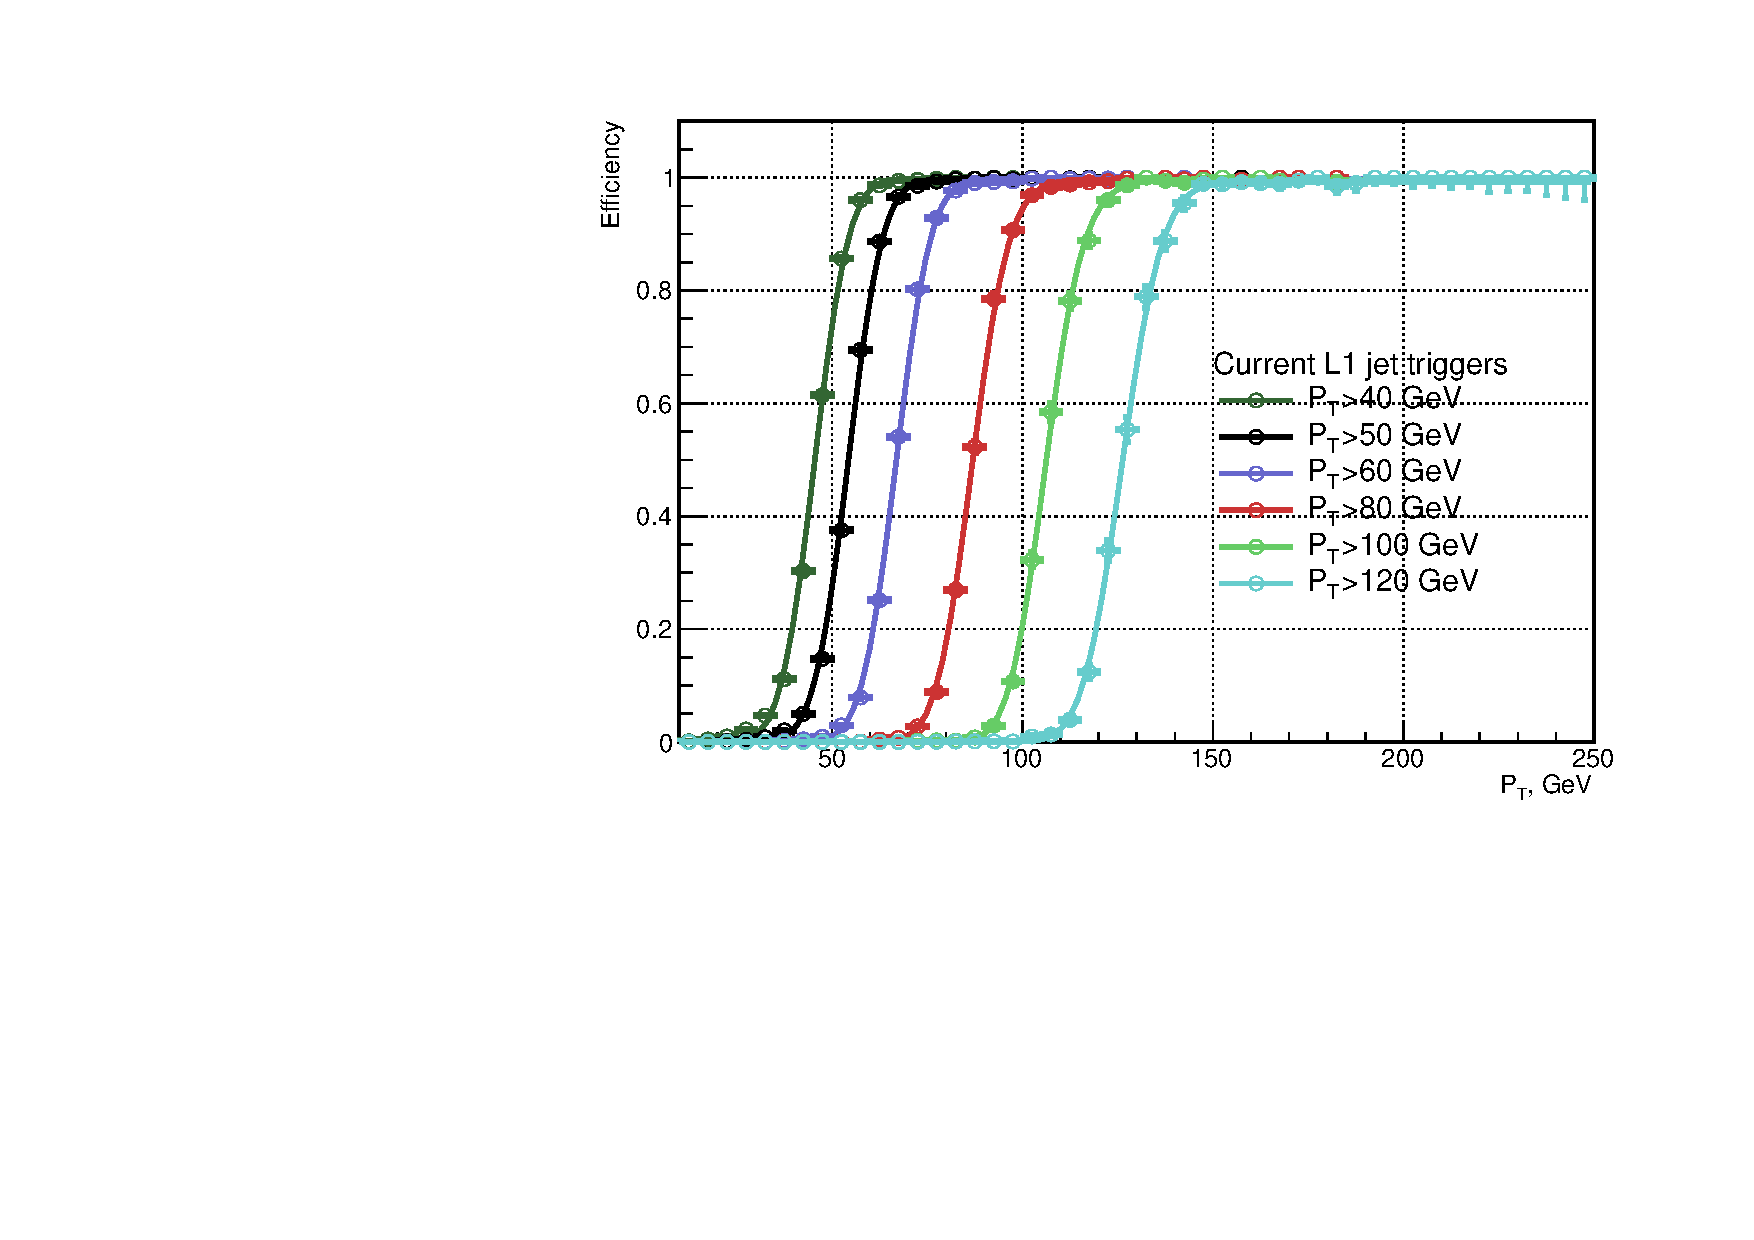
\includegraphics[scale=0.37]{Figures/l1jets//CurrentL1JetTriggers.pdf}
    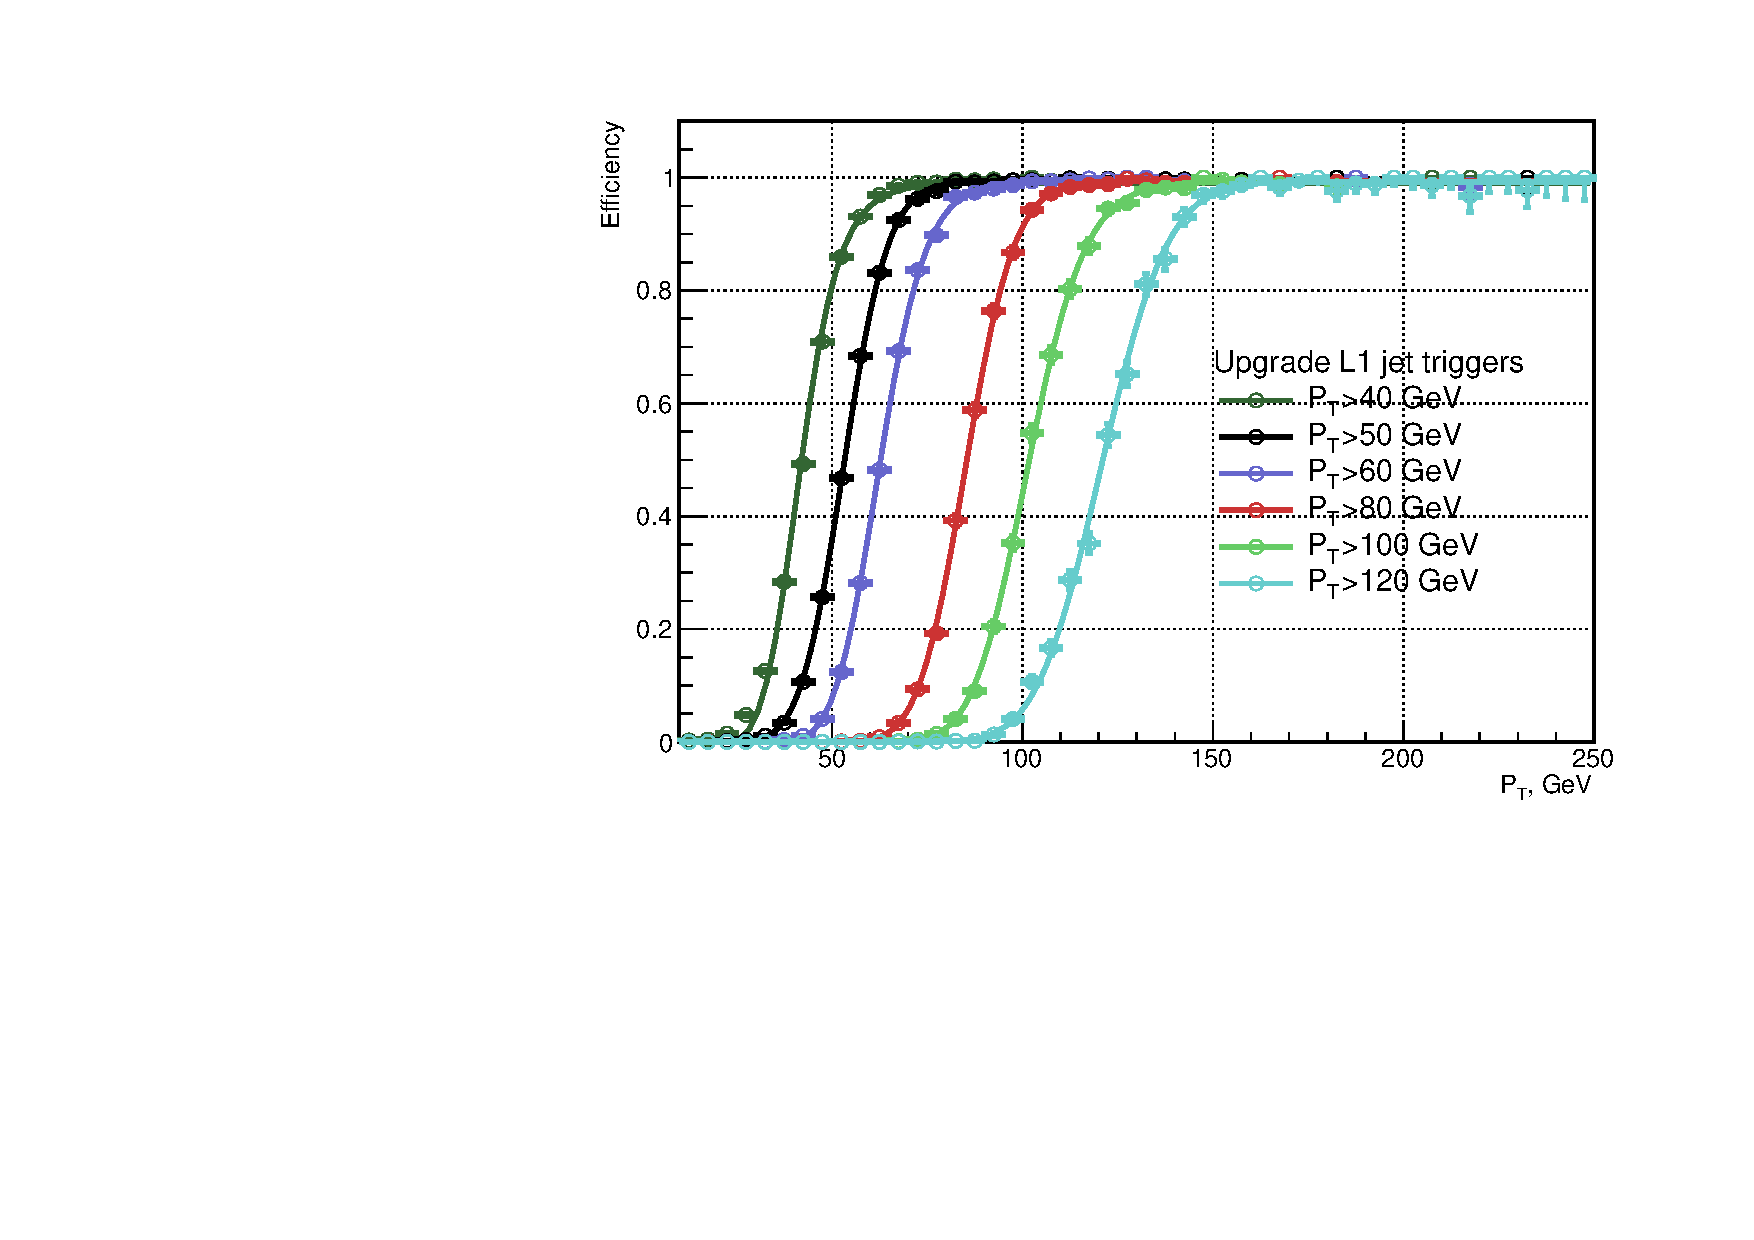
\includegraphics[scale=0.37]{Figures/l1jets//UpgradeL1JetTriggers.pdf}
\caption{On the left are the trigger turn on curves for the current jet algorithm and on the right are the trigger turn on curves for the upgrade jet algorithm, for various single jet trigger thresholds. These turn on curves were calculated using Single Muon 2012C data in PU normal PU conditions for 2012C running, ~20 primary vertices per event.}
\label{JetTO}
\end{center}
\end{figure}

\subsubsection{\sc Rates}
The L1 trigger is limited to the number events it can pass to the HLT. Triggers can only take a certain bandwidth; the sum of all trigger rates must be $\sim$ 300~kHz. 
In Zero Bias data, the rate at which the trigger would fire at a given L1 jet energy is calculated for a instantaneous luminosity scenario using the equation
\begin{equation}
\text{Rate}_{\text{Inst. lumi}} = \text{Rate}_{\text{event}} \cdot \frac{L\times \sigma_{pp}}{PU}
\end{equation}
Where $L$ is the instantaneous luminosity, $\sigma_{pp}$ is the proton-proton cross section and $PU$ is the number of vertices per bunch crossing.\\
Rates are plotted in terms of the 95\% threshold: physics groups set the cuts in analyses dependant on offline values at which trigger rates are $\geq 95\%$ efficient. Taking a set of turn on curves, such as those in Figure \ref{JetTO}, a linear conversion function between L1 threshold and 95\% threshold is attained.
Figure \ref{JetRate} shows the single and quad jet trigger rates. The current and upgrade single jet rates are comparable, as the PU subtraction does very little to the leading jet in the event, whereas the multi jet triggers such as the quad jet trigger sees a significant reduction in rate as PU jets are removed from the event.     


\begin{figure}[t!]
%\vspace{-1.cm}
\begin{center}
  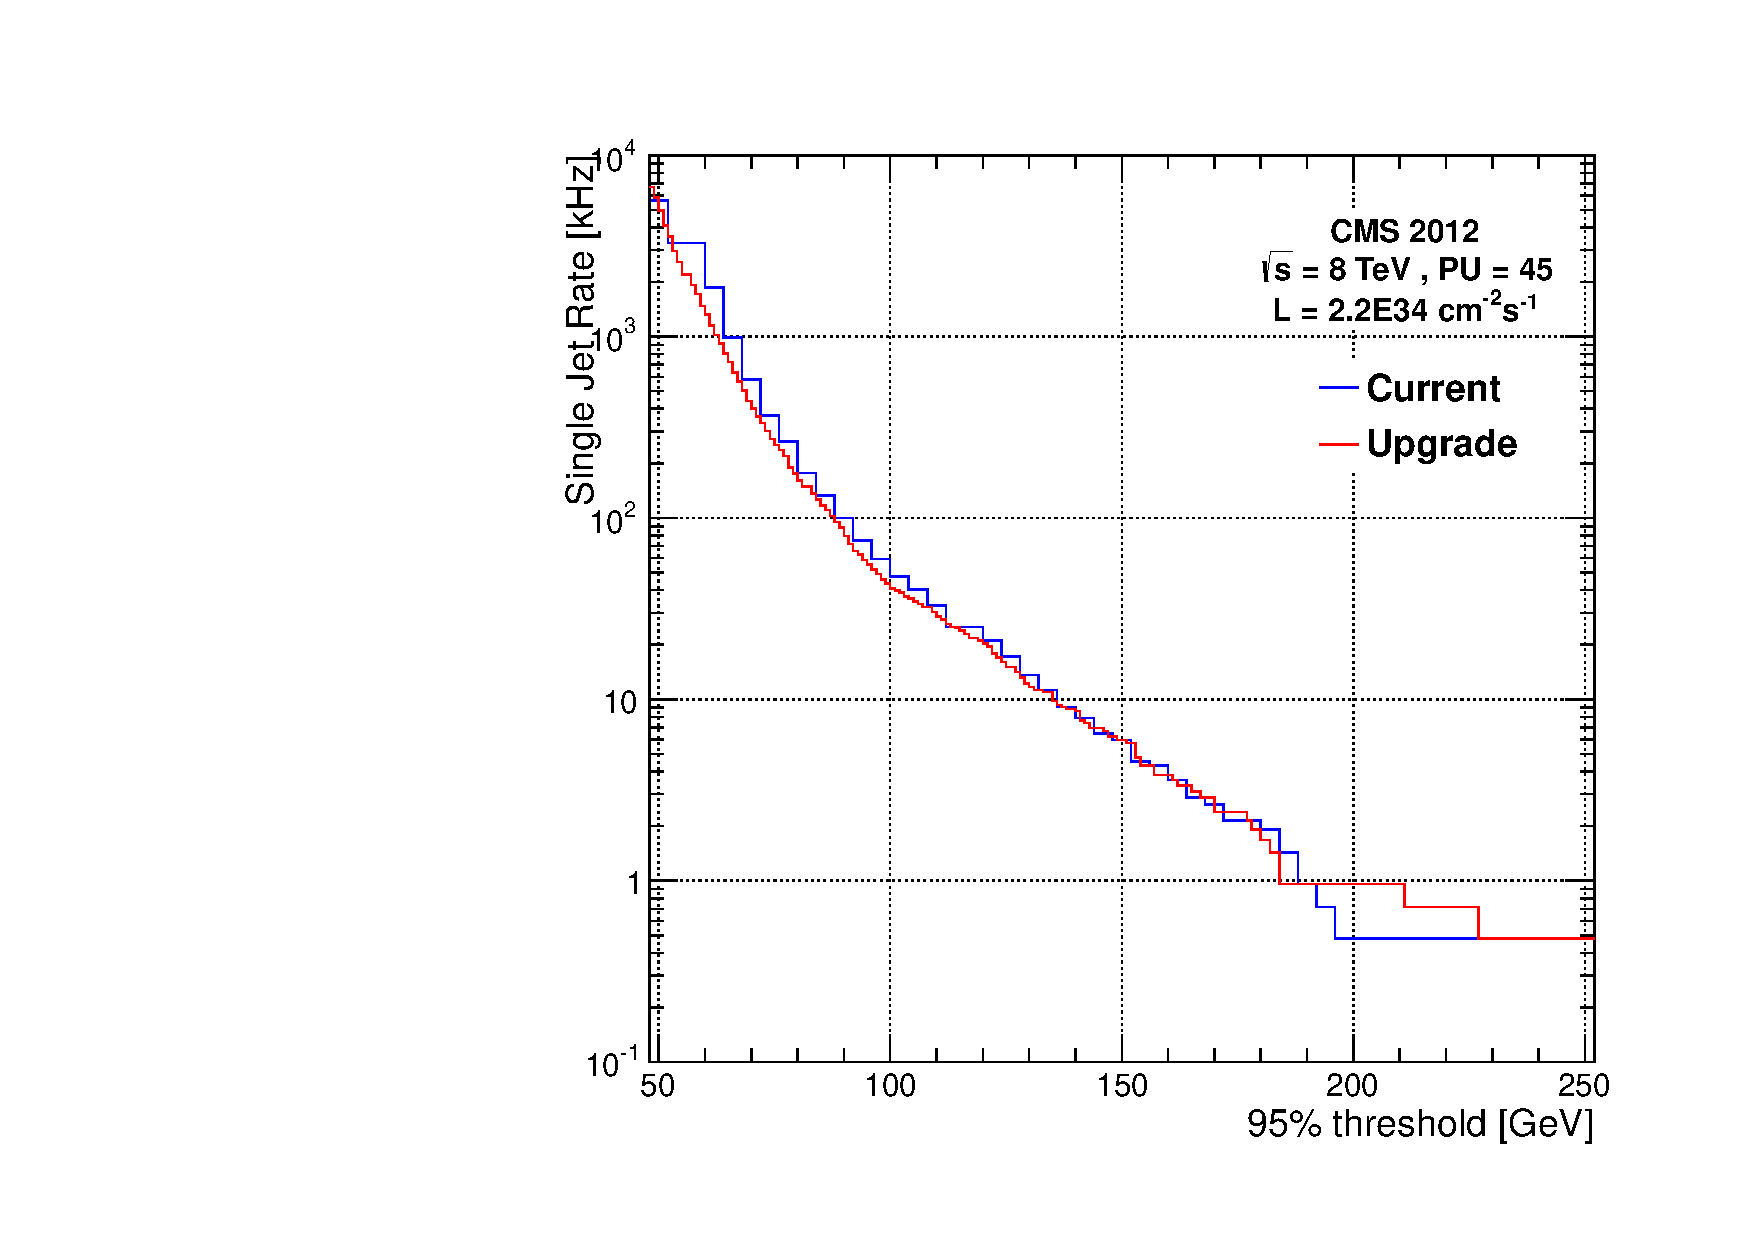
\includegraphics[scale=0.3]{Figures/l1jets/singleJetRates_95thresh_2e34.pdf}
    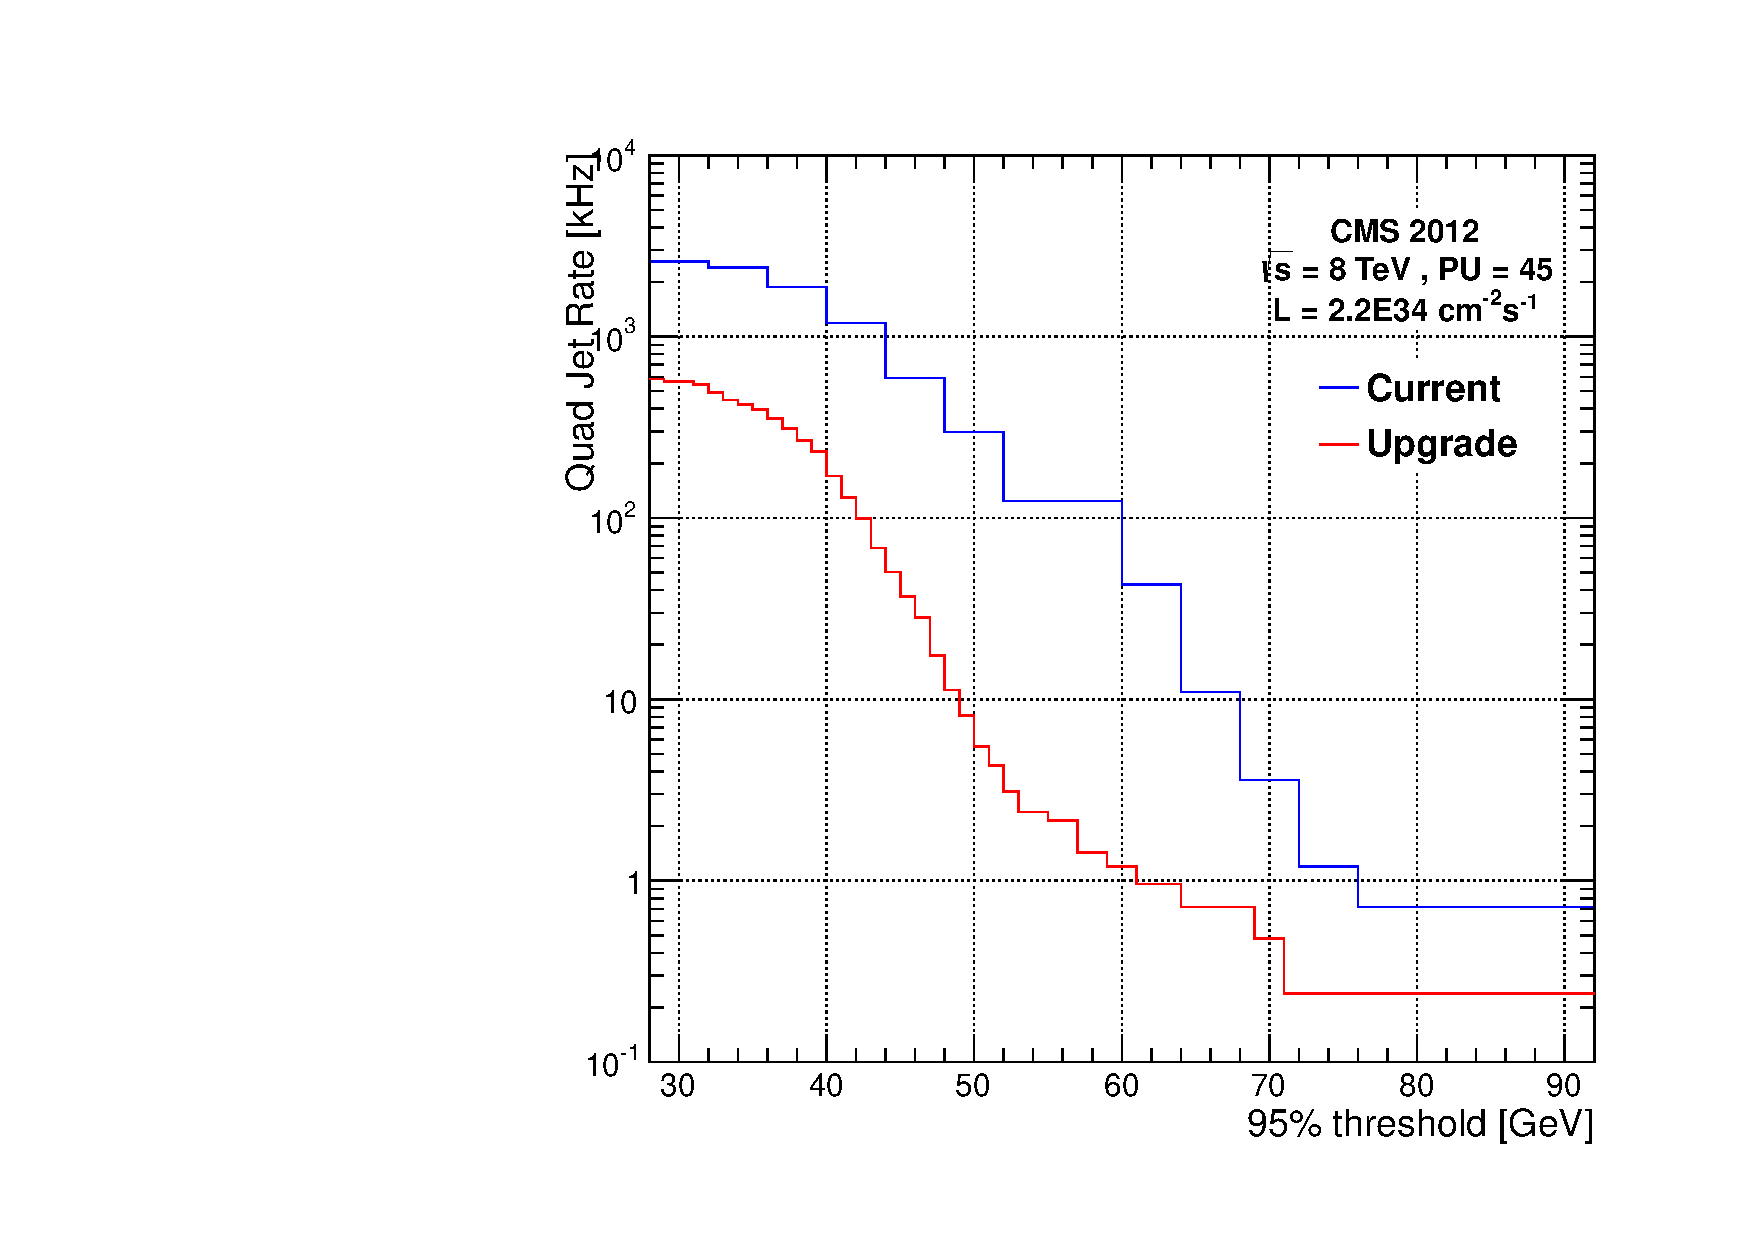
\includegraphics[scale=0.3]{Figures/l1jets/quadJetRates_95thresh_2e34.pdf}
\caption{Rates of single and quad jet triggers. The single jet trigger shows similar performance to the current system, while the multi-jet trigger show a large reduction in rate}
\label{JetRate}
\end{center}
\end{figure}
